\chapter{Methodology}
\label{chap:methodology}
\lhead{\emph{Problem Statement}}



\section{Introduction}



This chapter provides a comprehensive and detailed explanation of the techniques and procedures adopted during the course of the research. It serves to provide an in-depth account of the methods used in this study, thereby ensuring the research's transparency and reproducibility.

This research aims to enhance the performance of Optical Character Recognition (OCR) systems - specifically Tesseract OCR and Convolutional Recurrent Neural Network (CRNN) models - on images of sensor readings. To accomplish this, a systematic approach is adopted involving an initial global run of the OCR systems on the raw image datasets, followed by the application of specific image pre-processing techniques and subsequent localized OCR applications.

The purpose of these processes is to establish a baseline of OCR performance, then test the hypothesis that image pre-processing can enhance OCR results. The pre-processing, focused on applying colour masks before converting the images to grayscale, aims to increase the clarity of the images, thereby increasing the efficiency of the OCR processes.

This chapter outlines each of these processes in detail, thereby providing a clear roadmap of the research methodology adopted in this study. From the initial assessment of the OCR systems' performance to the implementation of the pre-processing techniques, this chapter serves as a guide to understanding the practical steps taken during this research project.

The subsequent sections provide further detail on the data being used, the OCR systems of focus, the pre-processing techniques applied, and the methods of evaluation. The goal of this chapter is to present a detailed and comprehensive account of the methodology that underpins this research.

---


\section{Data Collection}

The dataset used in this research was supplied as a collection of image files distributed across ten distinct folders. Each folder corresponds to a unique sensor from which readings were taken. These images provide a diversified dataset due to variations in sensor specifications and the conditions under which the readings were captured.

Upon receiving the data, an initial examination was carried out to ensure the integrity and completeness of the files. The image files were found to be in good condition, readable, and ready for further processing and analysis.

In order to streamline the data management and analysis process, a CSV file was created. This file serves as an inventory, containing each image file name and its corresponding label, thereby facilitating an efficient cross-referencing system for the data analysis phase.

To facilitate the training of the Convolutional Recurrent Neural Network (CRNN) models, multiple training databases were created. Each of these databases consists of 500,000 single digit training images, thereby providing a robust foundation for the machine learning tasks.

\newpage
\section{Data Analysis}

For each folder, there are three charts that provide an initial statistical data analysis of the images. These charts are as follows:


\begin{enumerate}
    \item \textbf{Montage:} A simple representation of the images in the folder, arranged in a grid format. This provides a visual overview of the images in the folder, thereby facilitating a quick assessment of the data.
    \item \textbf{RGB Histogram:} This chart shows the distribution of pixel intensities for the Red, Green, and Blue channels separately in each image.
          \begin{enumerate}

              \item \textit{Axes:} The X-axis represents the possible pixel intensity values (ranging from 0 to 255 for an 8-bit image), and the Y-axis represents the number of pixels in the image with that intensity value.
              \item \textit{Colour Lines:} The Red line shows the distribution of red pixel intensities, the Green line shows the distribution of green pixel intensities, and the Blue line shows the distribution of blue pixel intensities.
              \item \textit{Interpretation:} Peaks in the graph represent the colours that are most present in the image. For instance, a high peak in the red line around the value 200 would indicate that the image has many pixels with high red intensity, suggesting the image may visually appear reddish.
              \item \textit{Colour Composition:} The overall shape of these colour distributions can provide an idea about the colour composition of the images.
              \item \textit{Utility:} The RGB Histogram aids in understanding the dominant colours in the image, the contrast, and the brightness. Variations in these histograms across the image set might be related to different sensor readings or variations in image capture settings.
          \end{enumerate}
          \newpage
    \item \textbf{Data Analysis:} Eight metrics have been defined to quantify various properties of an image. Each of these metrics provides insight into different aspects of the image, allowing for a detailed analysis and comparison of images. These metrics are as follows:
          \begin{enumerate}

              \item \textbf{Contrast:} The Contrast chart visualizes the degree of local variation in an image, which can be associated with the details or changes in sensor readings.
              \item \textbf{Dissimilarity:} Dissimilarity, like contrast, measures local variations, offering additional information about changes in the image.
              \item \textbf{Homogeneity:} The Homogeneity chart shows the closeness of the distribution of elements in an image to its diagonal, providing insight into the uniformity or variation in sensor readings.
              \item \textbf{Energy:} The Energy chart encapsulates the sum of squared elements in the image, which can suggest patterns or randomness in sensor readings.
              \item \textbf{Correlation:} The Correlation chart illustrates the joint probability occurrence of specific pixel pairs, thereby hinting at the predictability or scatter of sensor readings.
              \item \textbf{Area:} The Area chart, in our context, represents the total area of contours detected in an image, providing information on the complexity of sensor readings.
              \item \textbf{Brightness:} The Brightness chart displays the average lightness or darkness of each image, which might be influenced by different environmental conditions or sensor settings.
              \item \textbf{Standard Deviation:} The Standard Deviation chart shows the variability in pixel intensities within each image, helping infer the contrast, detail, and complexity of sensor readings.
          \end{enumerate}


\end{enumerate}

\newpage

% \subsection{Folders}
\subsection{Sipa 2}

There are 167 JPEG files totalling a size of 15.78mb in this folder. The images are of varying dimensions.

\begin{figure}[ht]
    \centering
    \begin{minipage}[t]{0.25\textwidth}
        \centering
        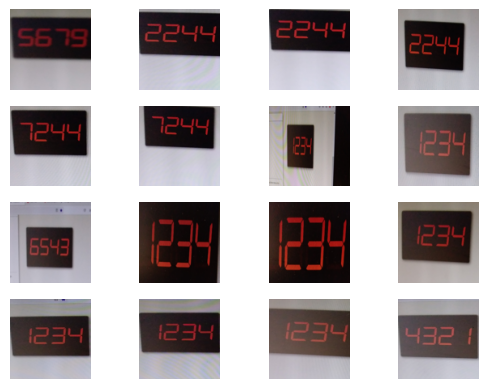
\includegraphics[width=\textwidth]{Figures/EDA_Charts/2/montage.png}
        \caption*{Montage}
    \end{minipage}\hfill
    \begin{minipage}[t]{0.25\textwidth}
        \centering
        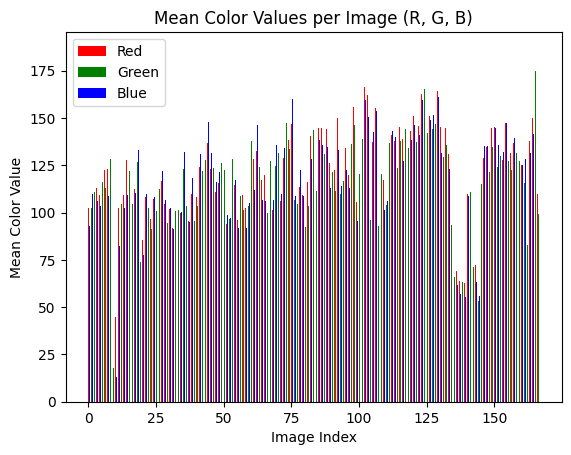
\includegraphics[width=\textwidth]{Figures/EDA_Charts/2/rgb.png}
        \caption*{RGB}
    \end{minipage}\hfill
    \begin{minipage}[t]{0.50\textwidth}
        \centering
        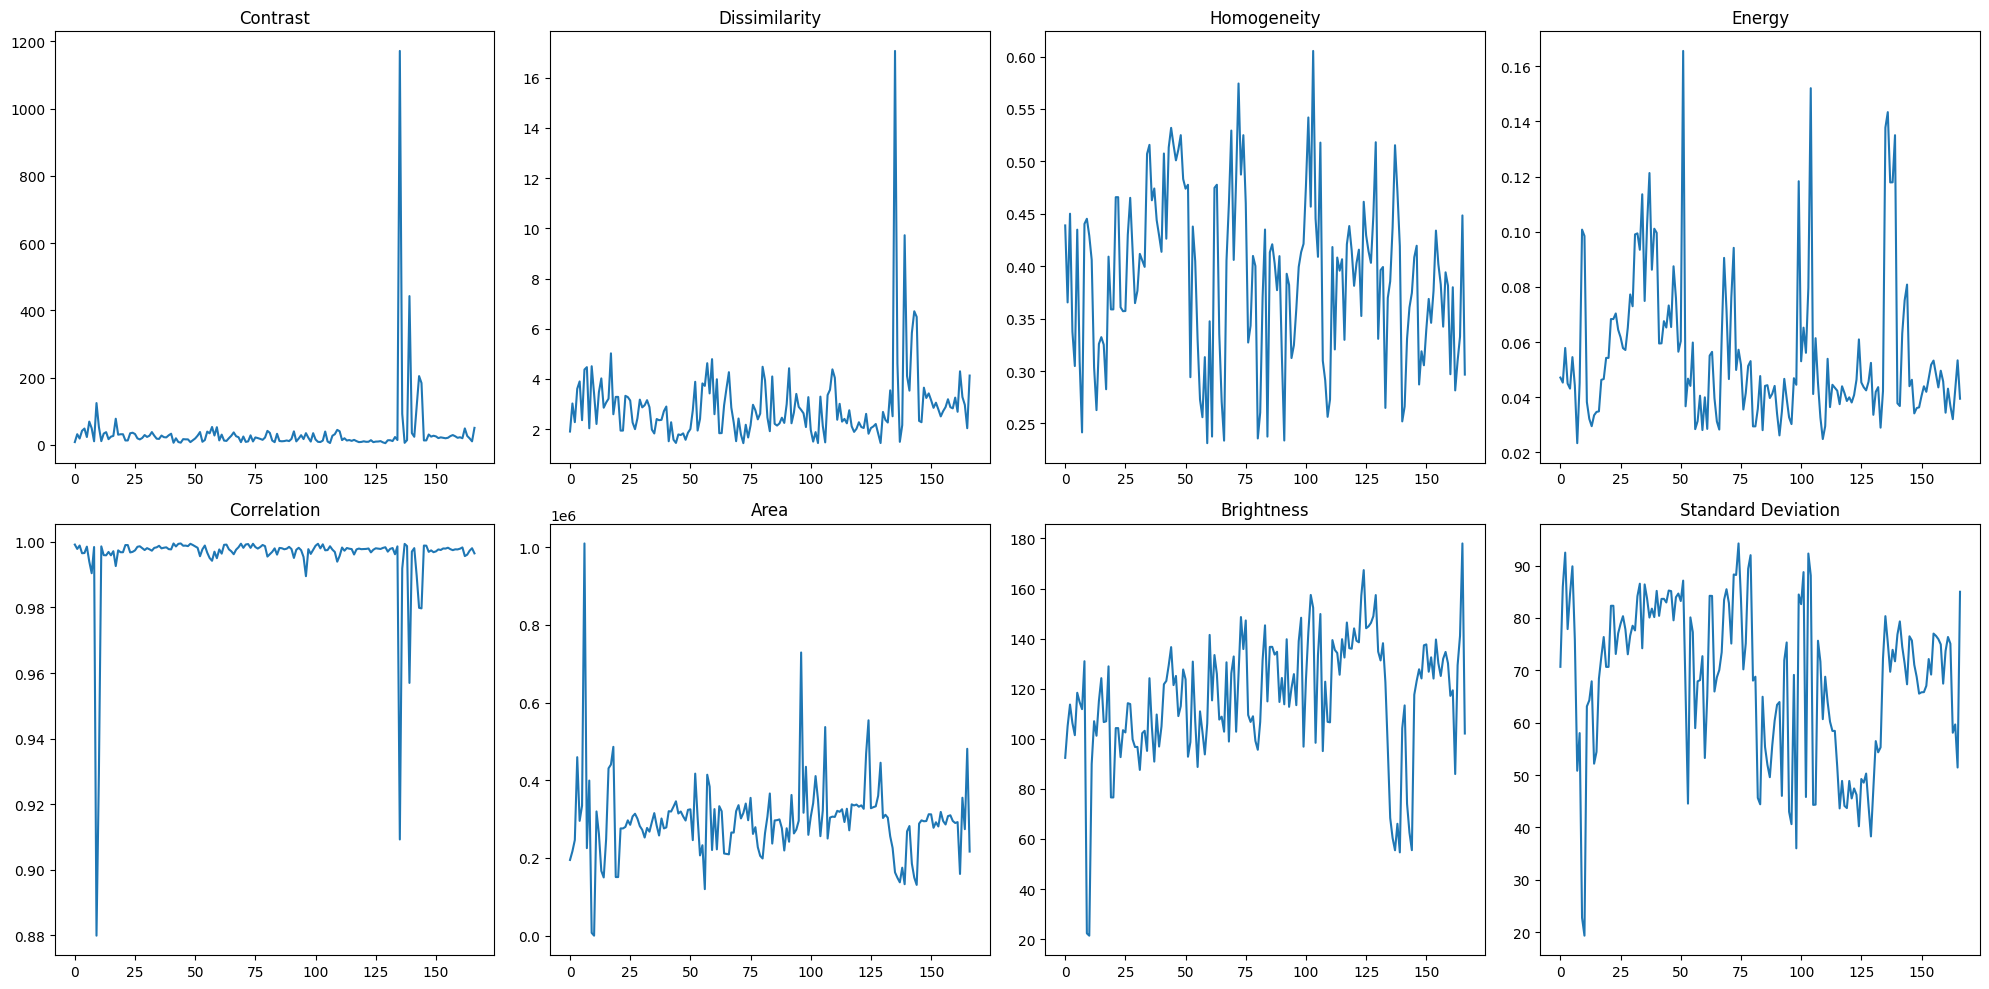
\includegraphics[width=\textwidth]{Figures/EDA_Charts/2/da.png}
        \caption*{Data Analysis}
    \end{minipage}
    \caption{Sipa 2 Analysis}
    \label{fig:Sipa 2 Analysis}
\end{figure}


\subsection{Sipa 3}

There are 26 JPEG files totalling a size of 77.88mb in this folder. The images are of varying dimensions.

\begin{figure}[ht]
    \centering
    \begin{minipage}[t]{0.25\textwidth}
        \centering
        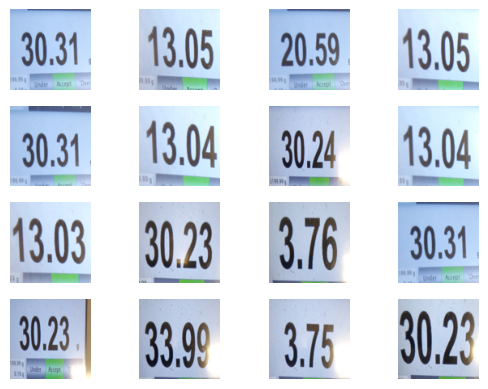
\includegraphics[width=\textwidth]{Figures/EDA_Charts/3/montage.png}
        \caption*{Montage}
    \end{minipage}\hfill
    \begin{minipage}[t]{0.25\textwidth}
        \centering
        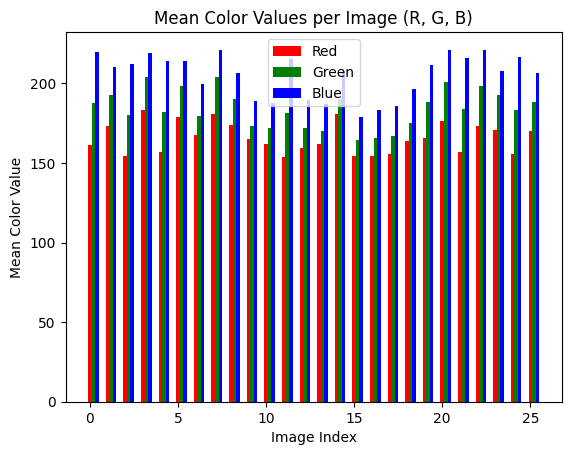
\includegraphics[width=\textwidth]{Figures/EDA_Charts/3/rgb.png}
        \caption*{RGB}
    \end{minipage}\hfill
    \begin{minipage}[t]{0.50\textwidth}
        \centering
        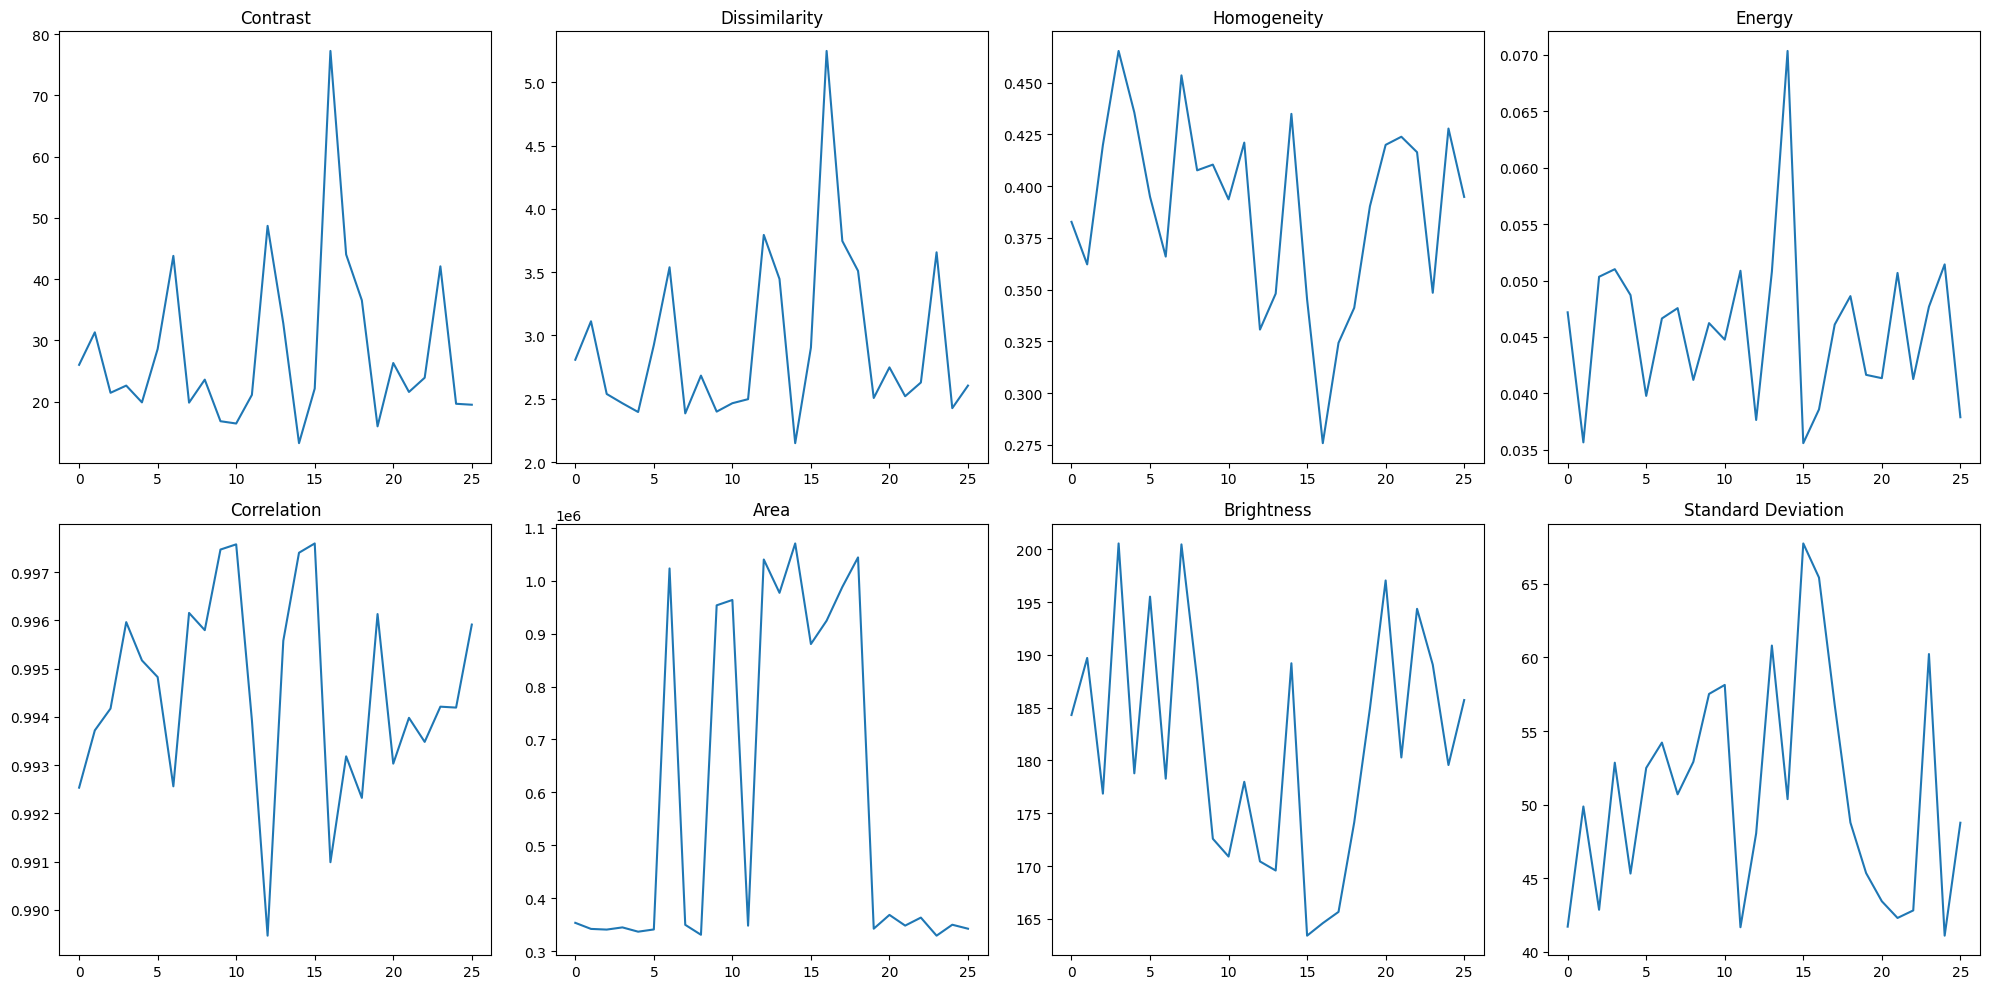
\includegraphics[width=\textwidth]{Figures/EDA_Charts/3/da.png}
        \caption*{Data Analysis}
    \end{minipage}
    \caption{Sipa 3 Analysis}
    \label{fig:Sipa 3 Analysis}
\end{figure}

\newpage

\subsection{Sipa 4}


There are 10 JPEG files totalling a size of 4.52mb in this folder. The images are of varying dimensions.

\begin{figure}[ht]
    \centering
    \begin{minipage}[t]{0.25\textwidth}
        \centering
        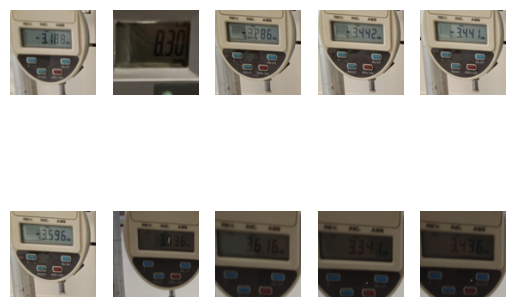
\includegraphics[width=\textwidth]{Figures/EDA_Charts/4/montage.png}
        \caption*{Montage}
    \end{minipage}\hfill
    \begin{minipage}[t]{0.25\textwidth}
        \centering
        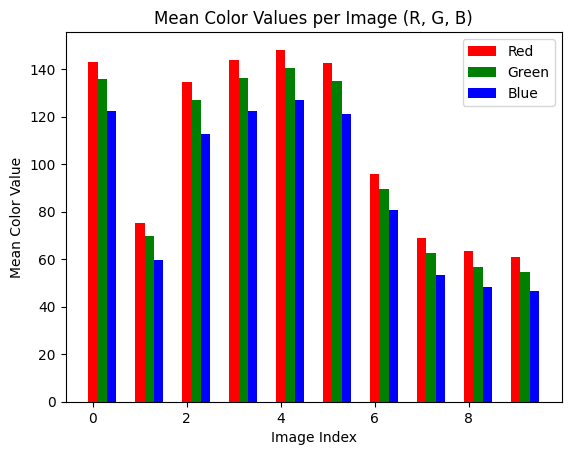
\includegraphics[width=\textwidth]{Figures/EDA_Charts/4/rgb.png}
        \caption*{RGB}
    \end{minipage}\hfill
    \begin{minipage}[t]{0.50\textwidth}
        \centering
        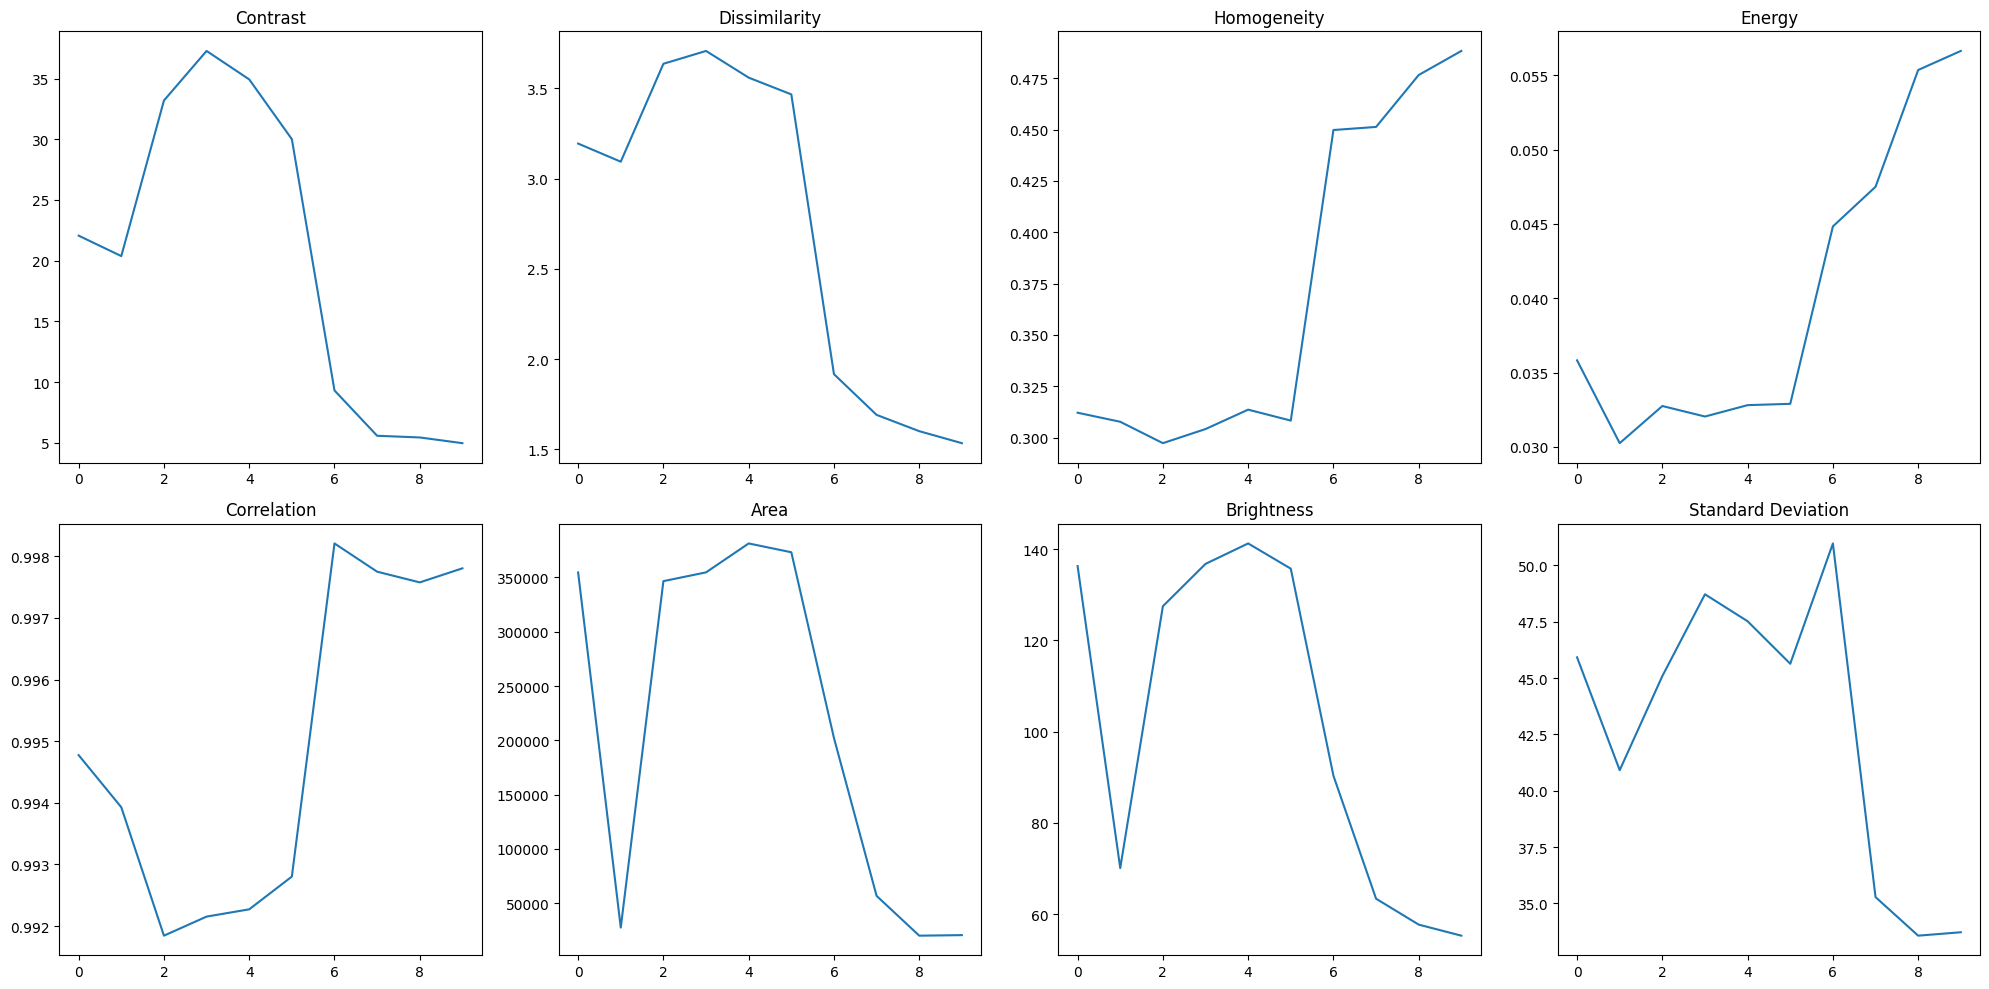
\includegraphics[width=\textwidth]{Figures/EDA_Charts/4/da.png}
        \caption*{Data Analysis}
    \end{minipage}
    \caption{Sipa 4 Analysis}
    \label{fig:Sipa 4 Analysis}
\end{figure}


\subsection{Sipa 5}

There are 27 JPEG files totalling a size of 6.96mb in this folder. The images are of varying dimensions.

\begin{figure}[ht]
    \centering
    \begin{minipage}[t]{0.25\textwidth}
        \centering
        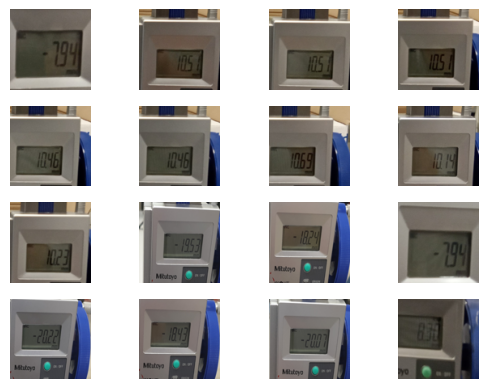
\includegraphics[width=\textwidth]{Figures/EDA_Charts/5/montage.png}
        \caption*{Montage}
    \end{minipage}\hfill
    \begin{minipage}[t]{0.25\textwidth}
        \centering
        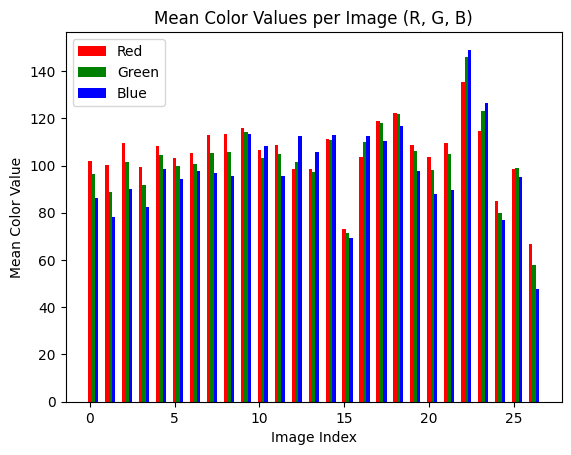
\includegraphics[width=\textwidth]{Figures/EDA_Charts/5/rgb.png}
        \caption*{RGB}
    \end{minipage}\hfill
    \begin{minipage}[t]{0.50\textwidth}
        \centering
        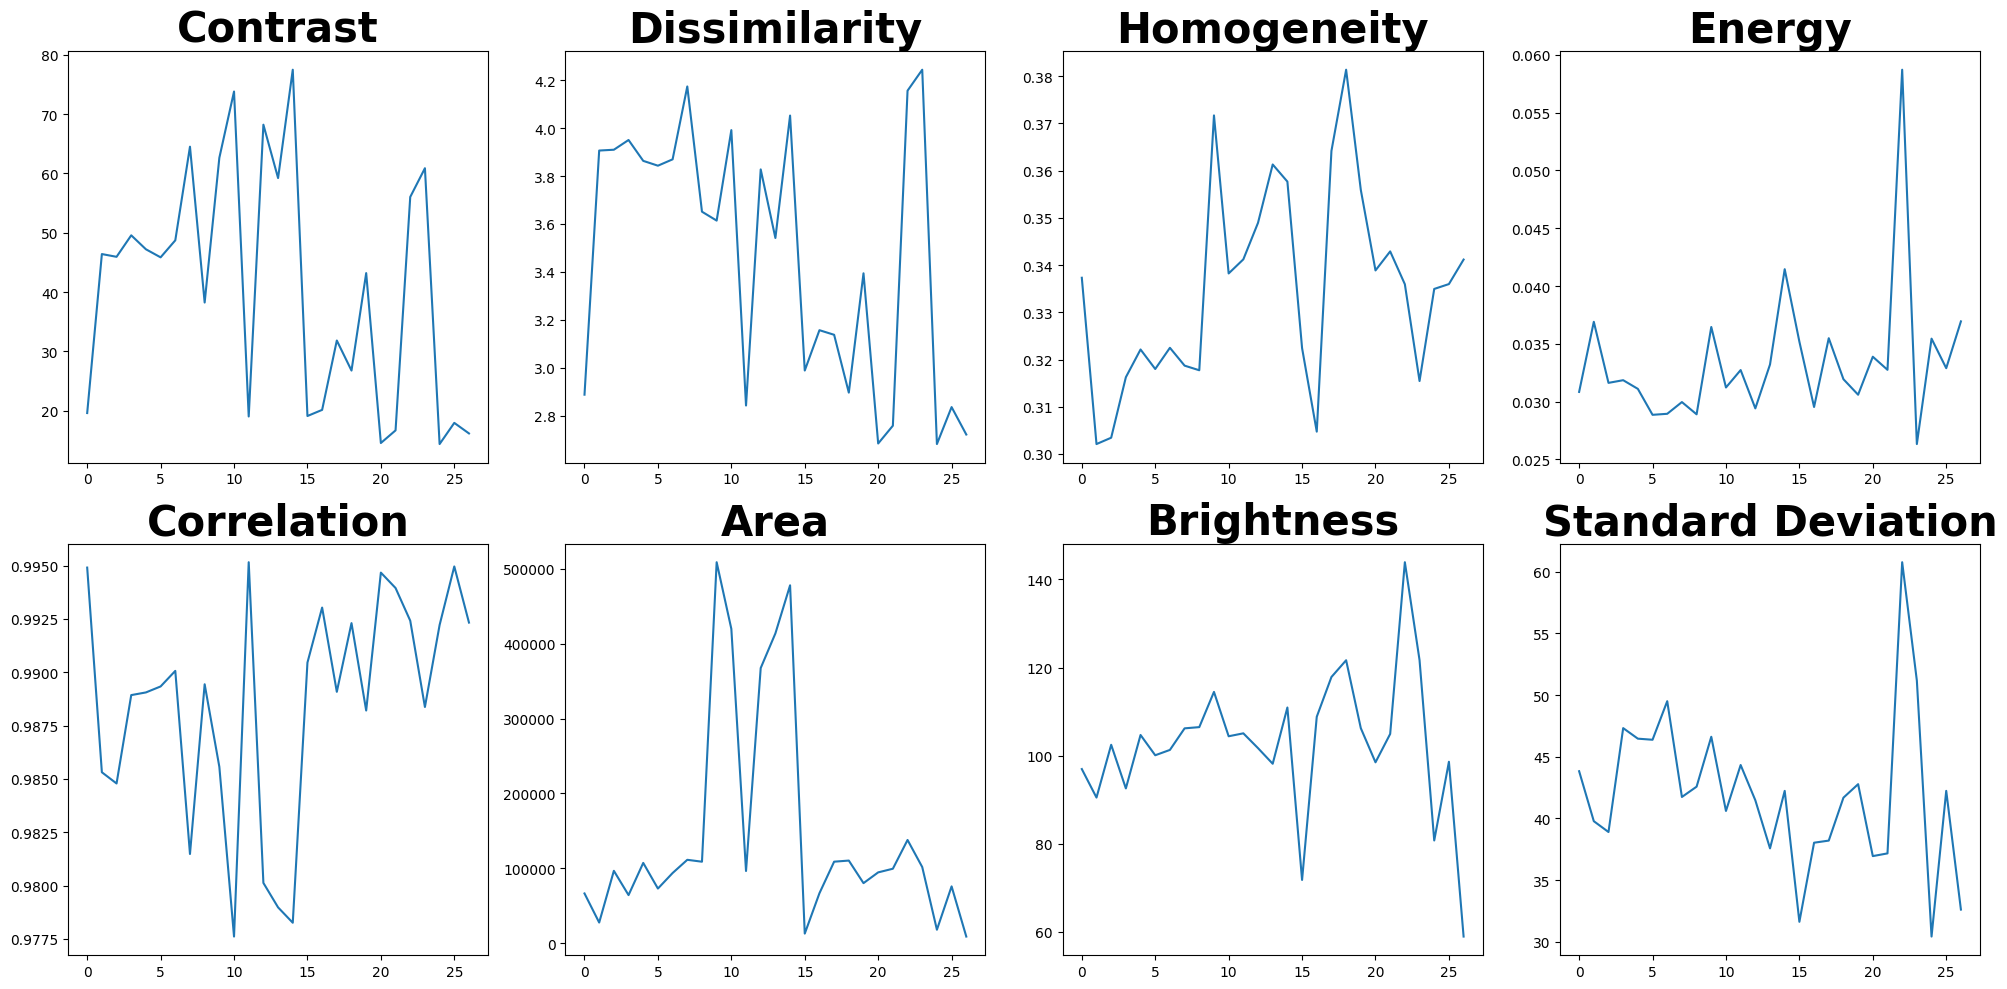
\includegraphics[width=\textwidth]{Figures/EDA_Charts/5/da.png}
        \caption*{Data Analysis}
    \end{minipage}
    \caption{Sipa 5 Analysis}
    \label{fig:Sipa 5 Analysis}
\end{figure}

\newpage

\subsection{Sipa 6}

There are 10 JPEG files totalling a size of 1.79mb in this folder. The images are of varying dimensions.

\begin{figure}[ht]
    \centering
    \begin{minipage}[t]{0.25\textwidth}
        \centering
        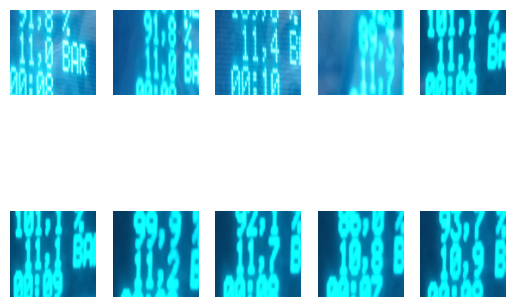
\includegraphics[width=\textwidth]{Figures/EDA_Charts/6/montage.png}
        \caption*{Montage}
    \end{minipage}\hfill
    \begin{minipage}[t]{0.25\textwidth}
        \centering
        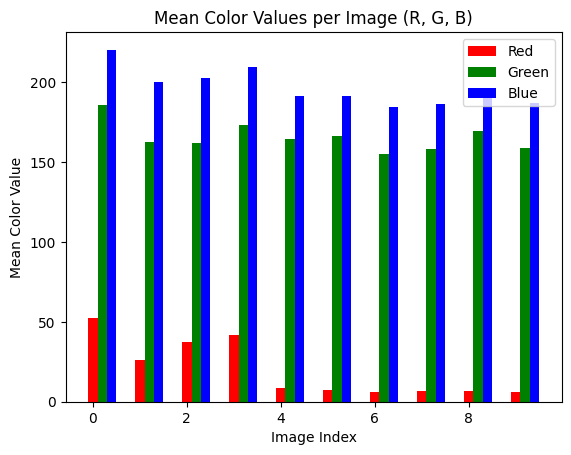
\includegraphics[width=\textwidth]{Figures/EDA_Charts/6/rgb.png}
        \caption*{RGB}
    \end{minipage}\hfill
    \begin{minipage}[t]{0.50\textwidth}
        \centering
        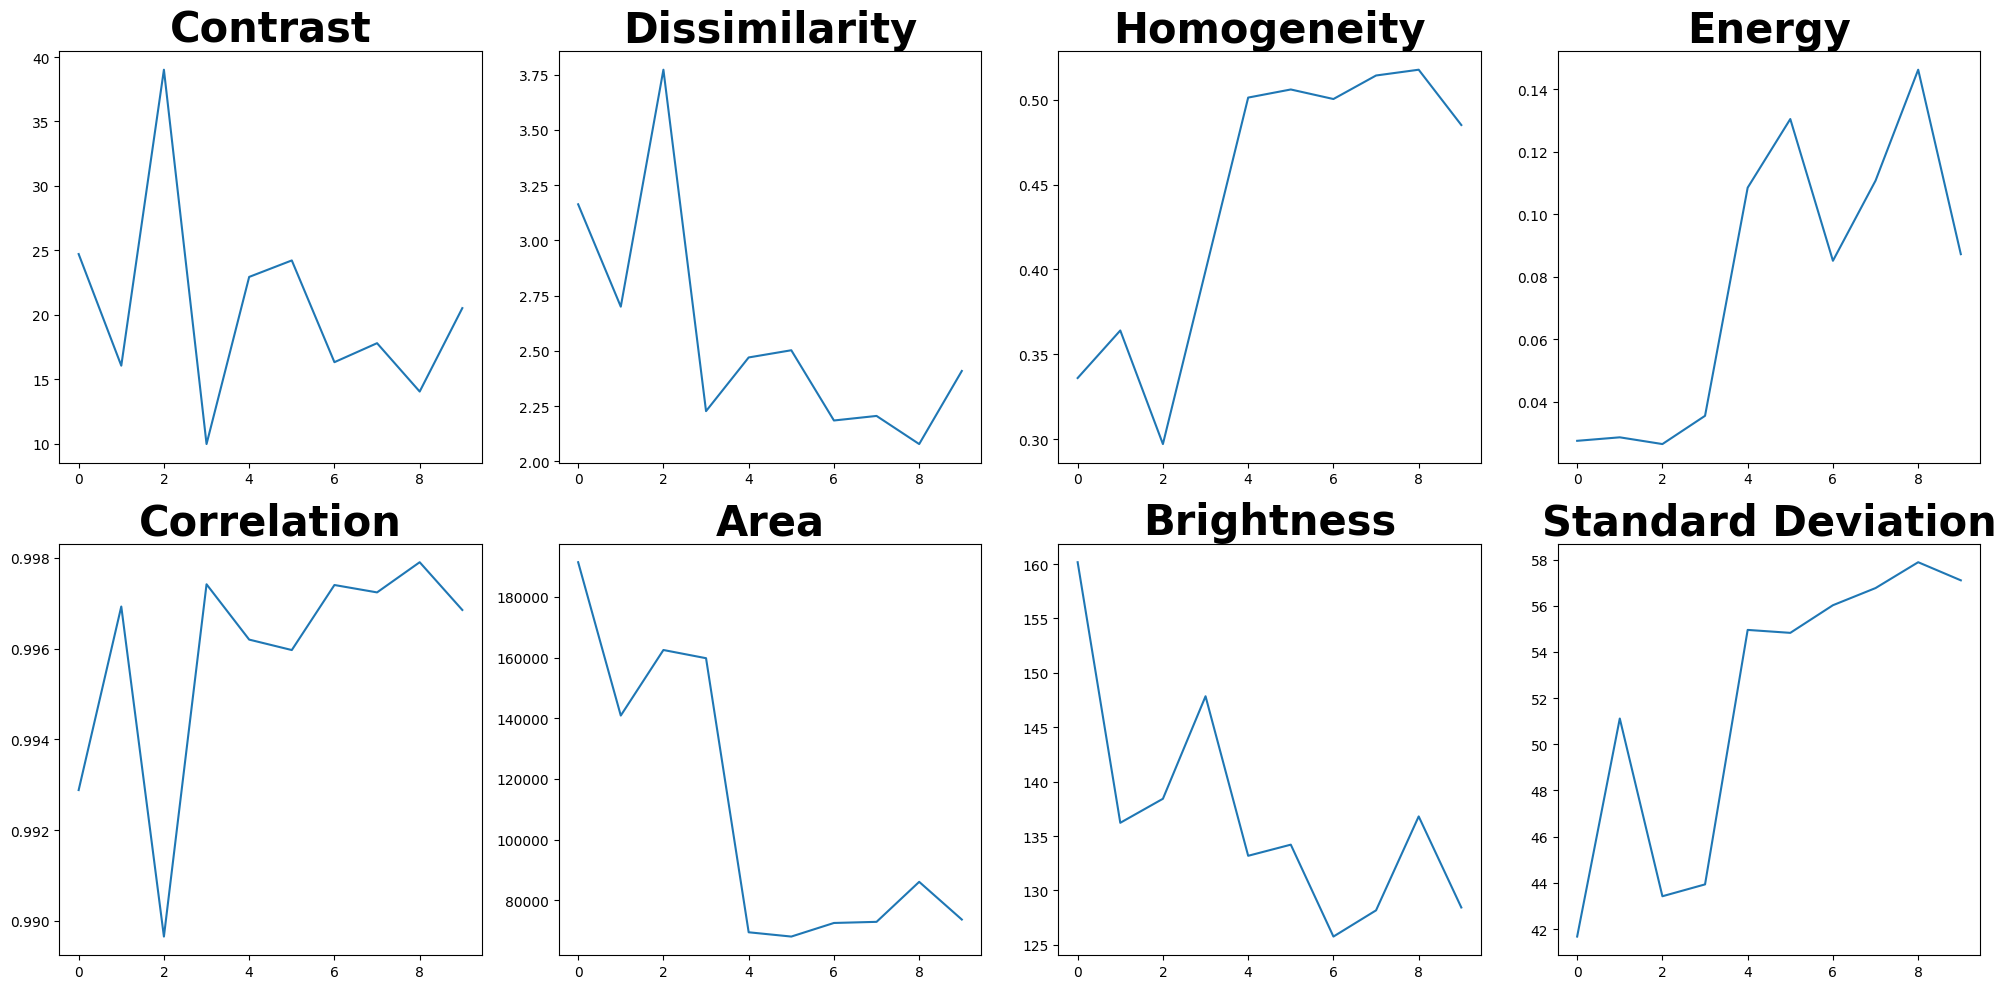
\includegraphics[width=\textwidth]{Figures/EDA_Charts/6/da.png}
        \caption*{Data Analysis}
    \end{minipage}
    \caption{Sipa 6 Analysis}
    \label{fig:Sipa 6 Analysis}
\end{figure}


\subsection{Sipa 7}

There are 10 JPEG files totalling a size of 4.98mb in this folder. The images are of varying dimensions.


\begin{figure}[ht]
    \centering
    \begin{minipage}[t]{0.25\textwidth}
        \centering
        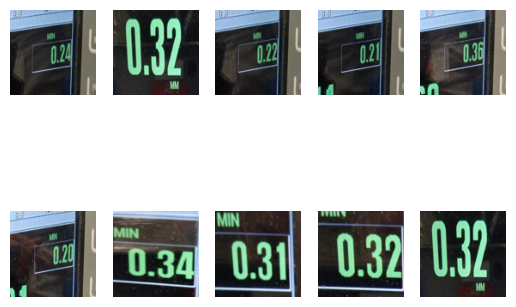
\includegraphics[width=\textwidth]{Figures/EDA_Charts/7/montage.png}
        \caption*{Montage}
    \end{minipage}\hfill
    \begin{minipage}[t]{0.25\textwidth}
        \centering
        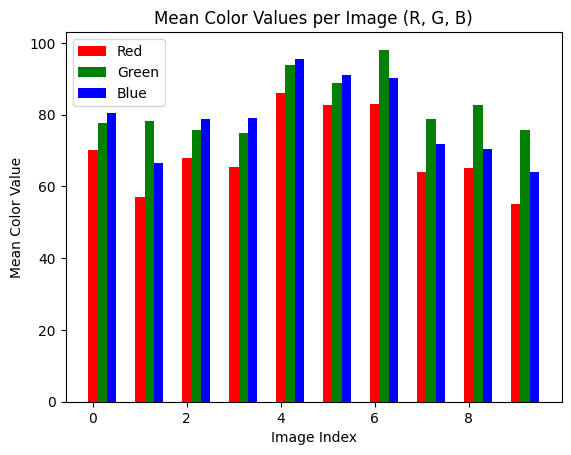
\includegraphics[width=\textwidth]{Figures/EDA_Charts/7/rgb.png}
        \caption*{RGB}
    \end{minipage}\hfill
    \begin{minipage}[t]{0.50\textwidth}
        \centering
        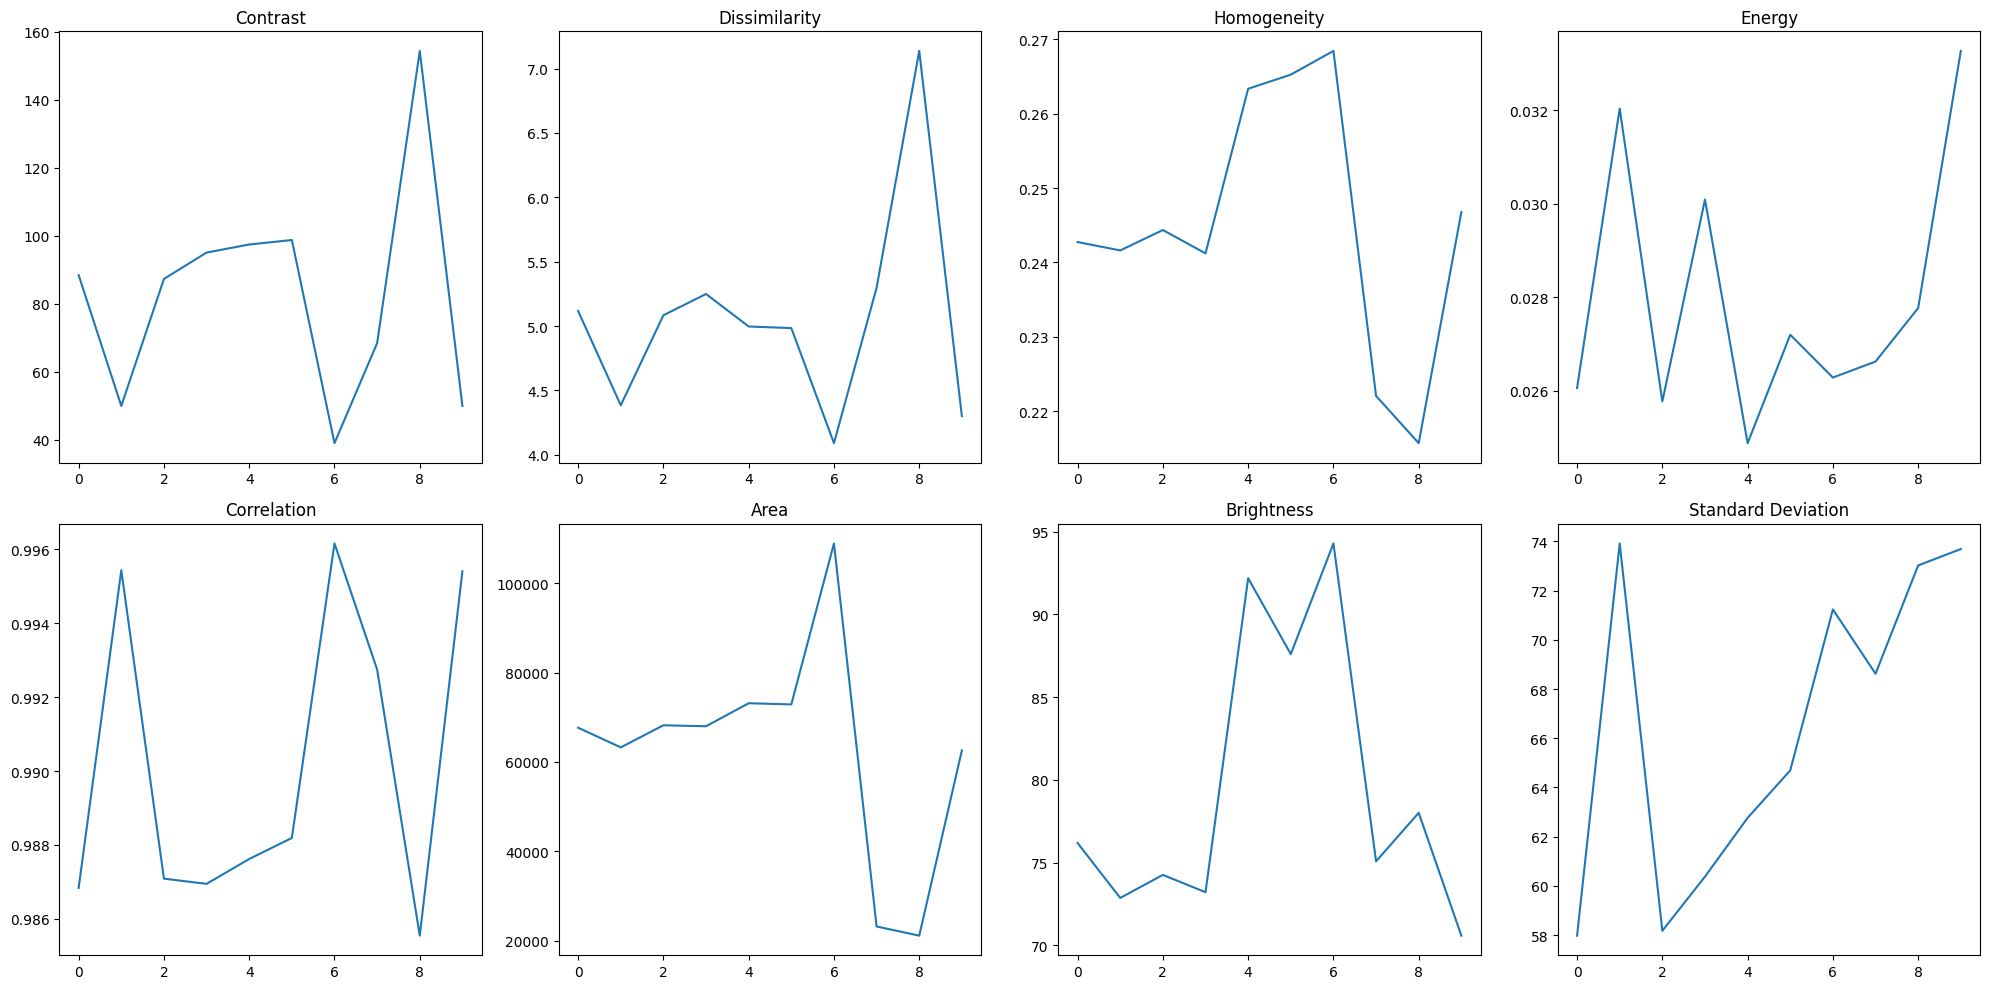
\includegraphics[width=\textwidth]{Figures/EDA_Charts/7/da.png}
        \caption*{Data Analysis}
    \end{minipage}
    \caption{Sipa 7 Analysis}
    \label{fig:Sipa 7 Analysis}
\end{figure}

\newpage

\subsection{Sipa 8}

There are 15 JPEG files totalling a size of 5.93mb in this folder. The images are of varying dimensions.


\begin{figure}[ht]
    \centering
    \begin{minipage}[t]{0.25\textwidth}
        \centering
        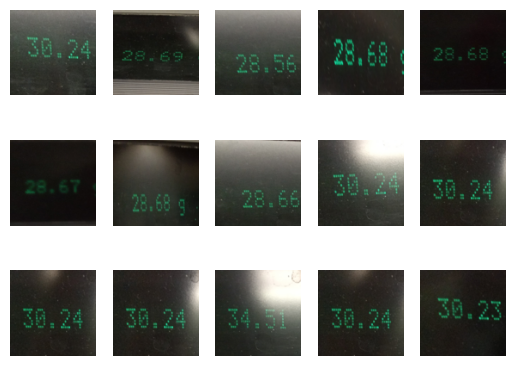
\includegraphics[width=\textwidth]{Figures/EDA_Charts/8/montage.png}
        \caption*{Montage}
    \end{minipage}\hfill
    \begin{minipage}[t]{0.25\textwidth}
        \centering
        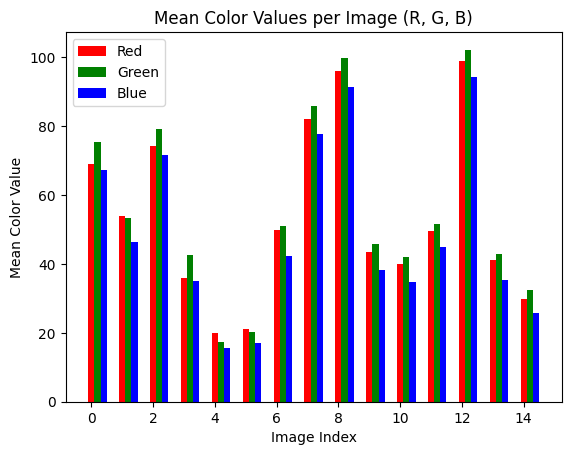
\includegraphics[width=\textwidth]{Figures/EDA_Charts/8/rgb.png}
        \caption*{RGB}
    \end{minipage}\hfill
    \begin{minipage}[t]{0.50\textwidth}
        \centering
        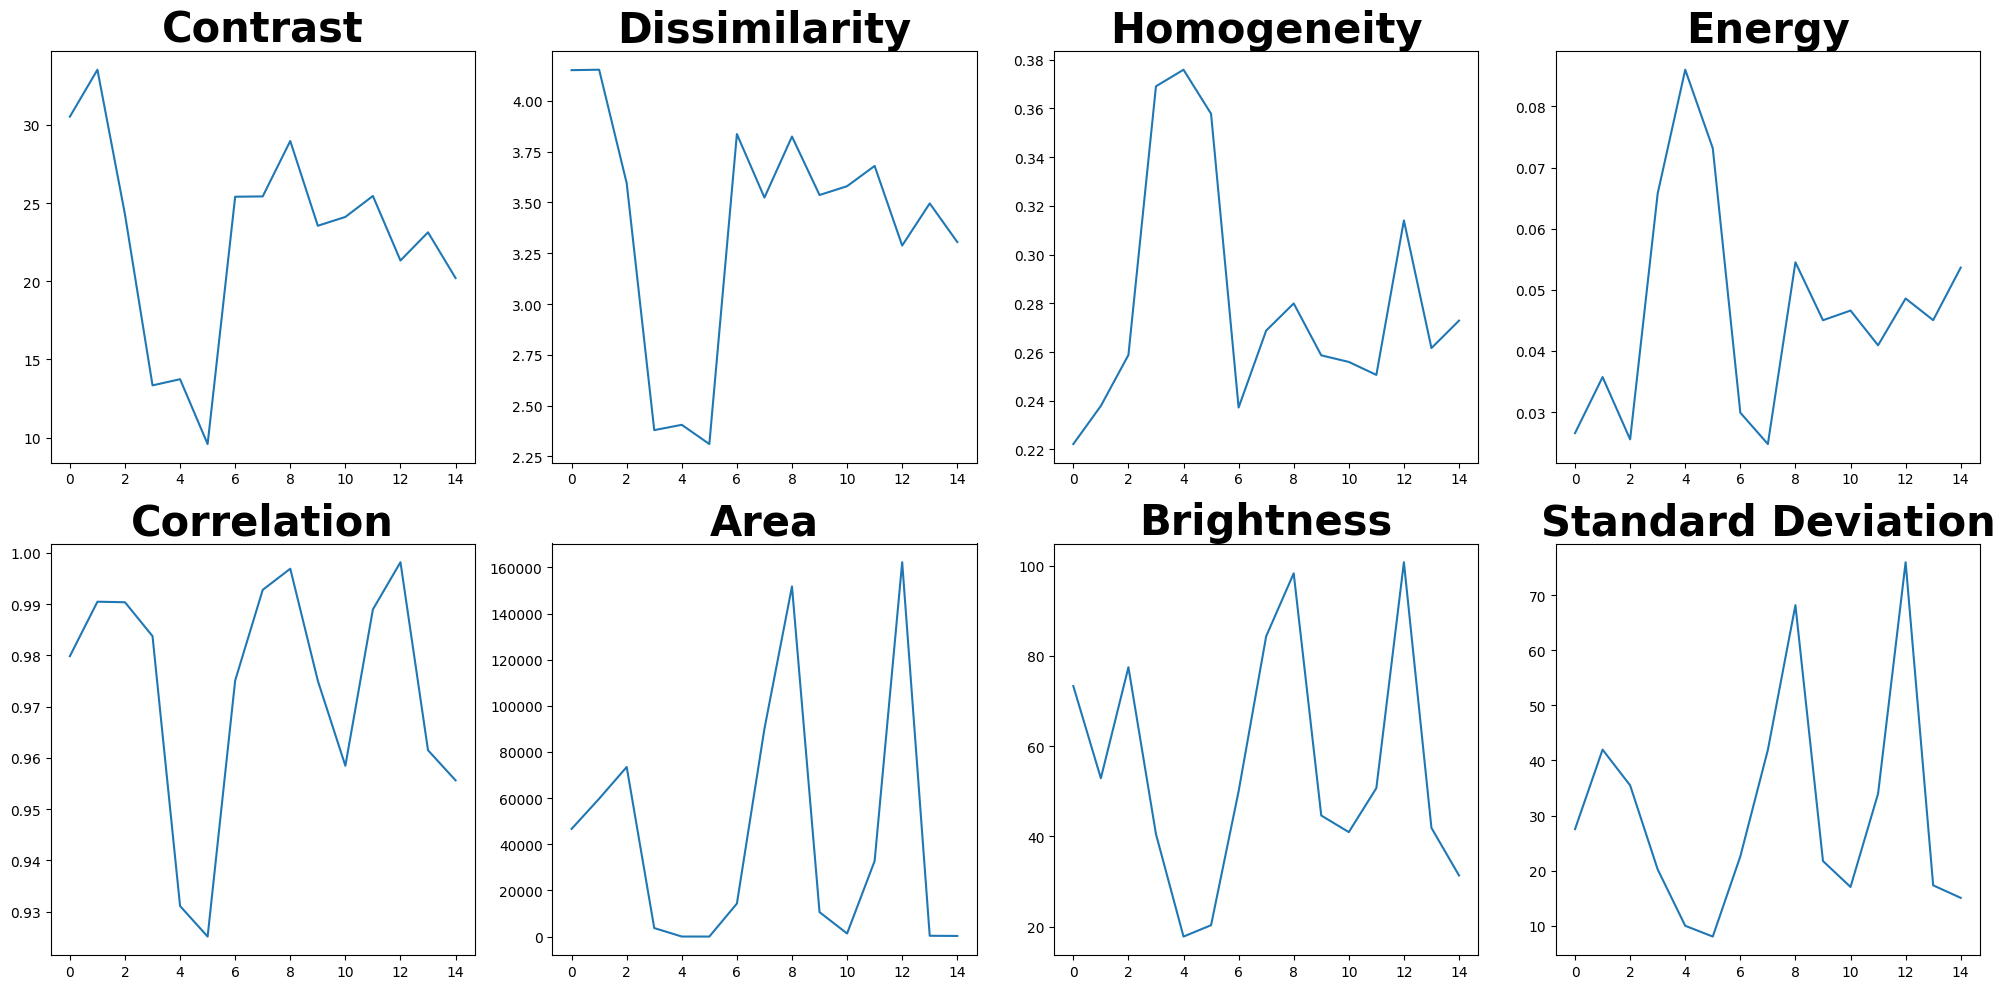
\includegraphics[width=\textwidth]{Figures/EDA_Charts/8/da.png}
        \caption*{Data Analysis}
    \end{minipage}
    \caption{Sipa 8 Analysis}
    \label{fig:Sipa 8 Analysis}
\end{figure}

\subsection{Sipa 9}

There are 12 JPEG files totalling a size of 7.34mb in this folder. The images are of varying dimensions.


\begin{figure}[ht]
    \centering
    \begin{minipage}[t]{0.25\textwidth}
        \centering
        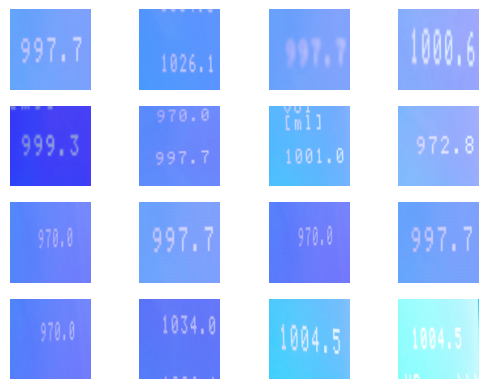
\includegraphics[width=\textwidth]{Figures/EDA_Charts/9/montage.png}
        \caption*{Montage}
    \end{minipage}\hfill
    \begin{minipage}[t]{0.25\textwidth}
        \centering
        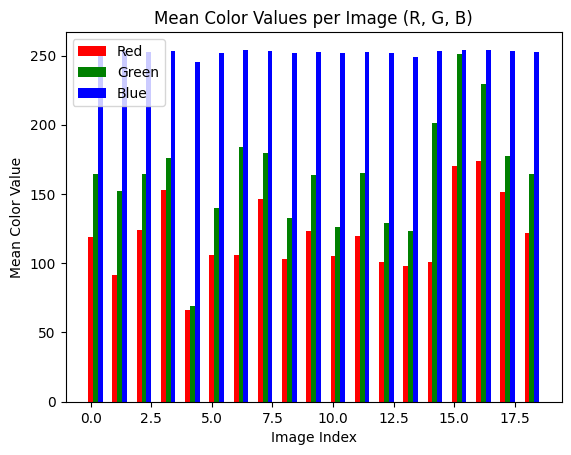
\includegraphics[width=\textwidth]{Figures/EDA_Charts/9/rgb.png}
        \caption*{RGB}
    \end{minipage}\hfill
    \begin{minipage}[t]{0.50\textwidth}
        \centering
        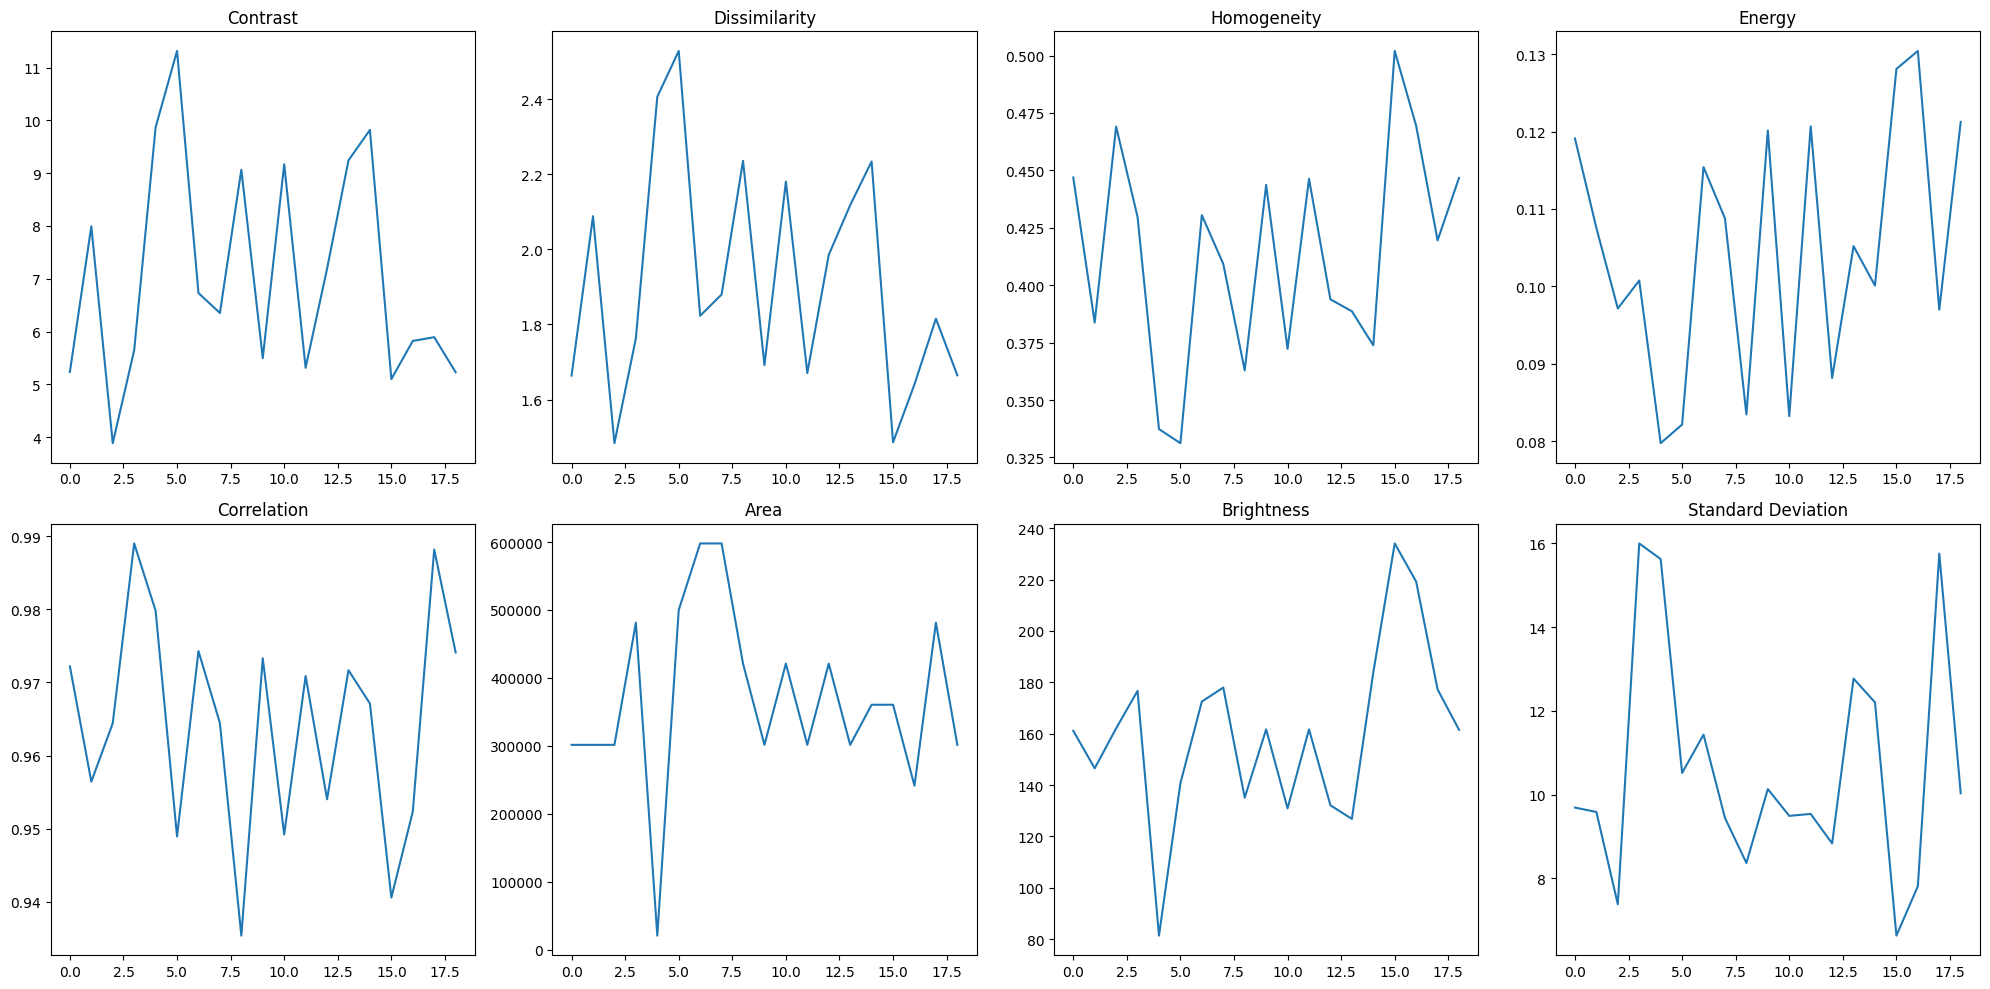
\includegraphics[width=\textwidth]{Figures/EDA_Charts/9/da.png}
        \caption*{Data Analysis}
    \end{minipage}
    \caption{Sipa 9 Analysis}
    \label{fig:Sipa 9 Analysis}
\end{figure}

\newpage

\subsection{Sipa 10}

There are 6 JPEG files totalling a size of 3.36mb in this folder. The images are of varying dimensions.


\begin{figure}[ht]
    \centering
    \begin{minipage}[t]{0.25\textwidth}
        \centering
        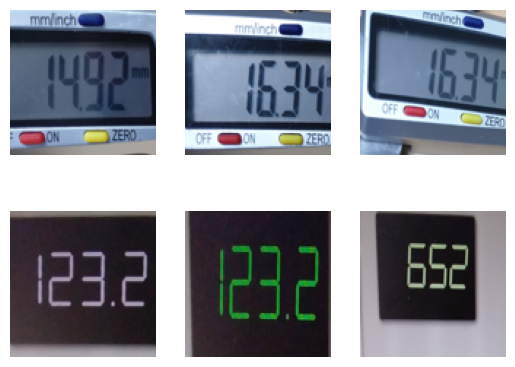
\includegraphics[width=\textwidth]{Figures/EDA_Charts/10/montage.png}
        \caption*{Montage}
    \end{minipage}\hfill
    \begin{minipage}[t]{0.25\textwidth}
        \centering
        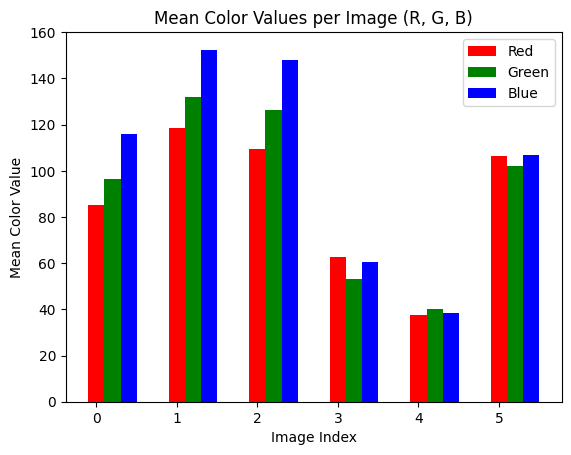
\includegraphics[width=\textwidth]{Figures/EDA_Charts/10/rgb.png}
        \caption*{RGB}
    \end{minipage}\hfill
    \begin{minipage}[t]{0.50\textwidth}
        \centering
        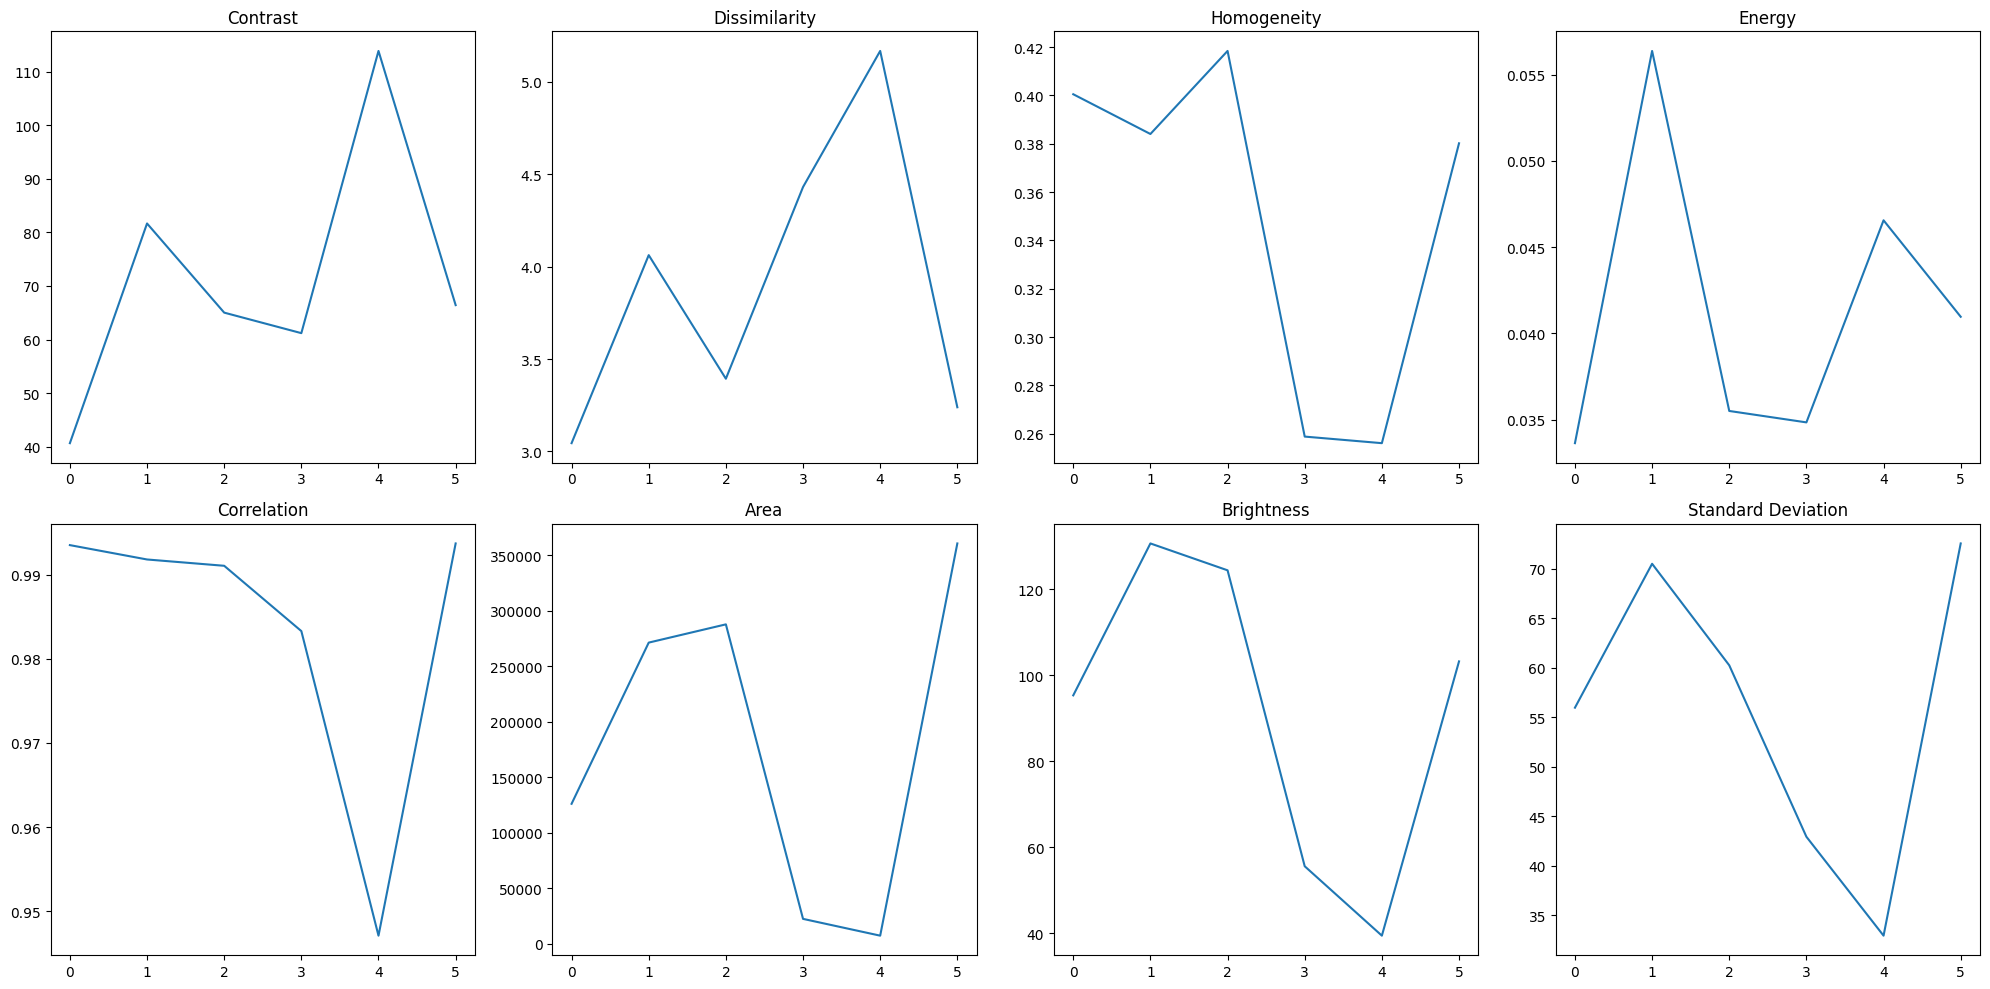
\includegraphics[width=\textwidth]{Figures/EDA_Charts/10/da.png}
        \caption*{Data Analysis}
    \end{minipage}
    \caption{Sipa 10 Analysis}
    \label{fig:Sipa 10 Analysis}
\end{figure}


\subsection{Sipa 11}

There are 14 JPEG files totalling a size of 6.16mb in this folder. The images are of varying dimensions.


\begin{figure}[ht]
    \centering
    \begin{minipage}[t]{0.25\textwidth}
        \centering
        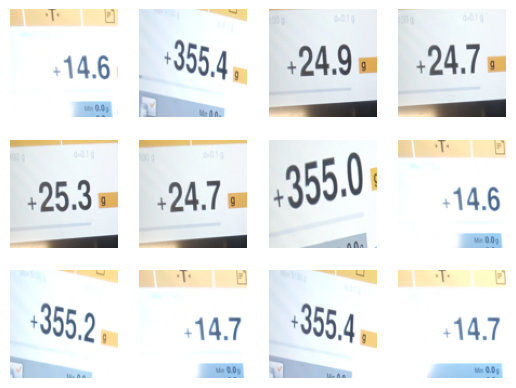
\includegraphics[width=\textwidth]{Figures/EDA_Charts/11/montage.png}
        \caption*{Montage}
    \end{minipage}\hfill
    \begin{minipage}[t]{0.25\textwidth}
        \centering
        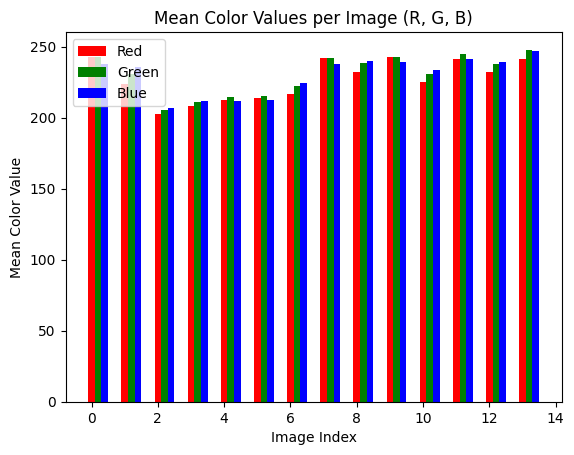
\includegraphics[width=\textwidth]{Figures/EDA_Charts/11/rgb.png}
        \caption*{RGB}
    \end{minipage}\hfill
    \begin{minipage}[t]{0.50\textwidth}
        \centering
        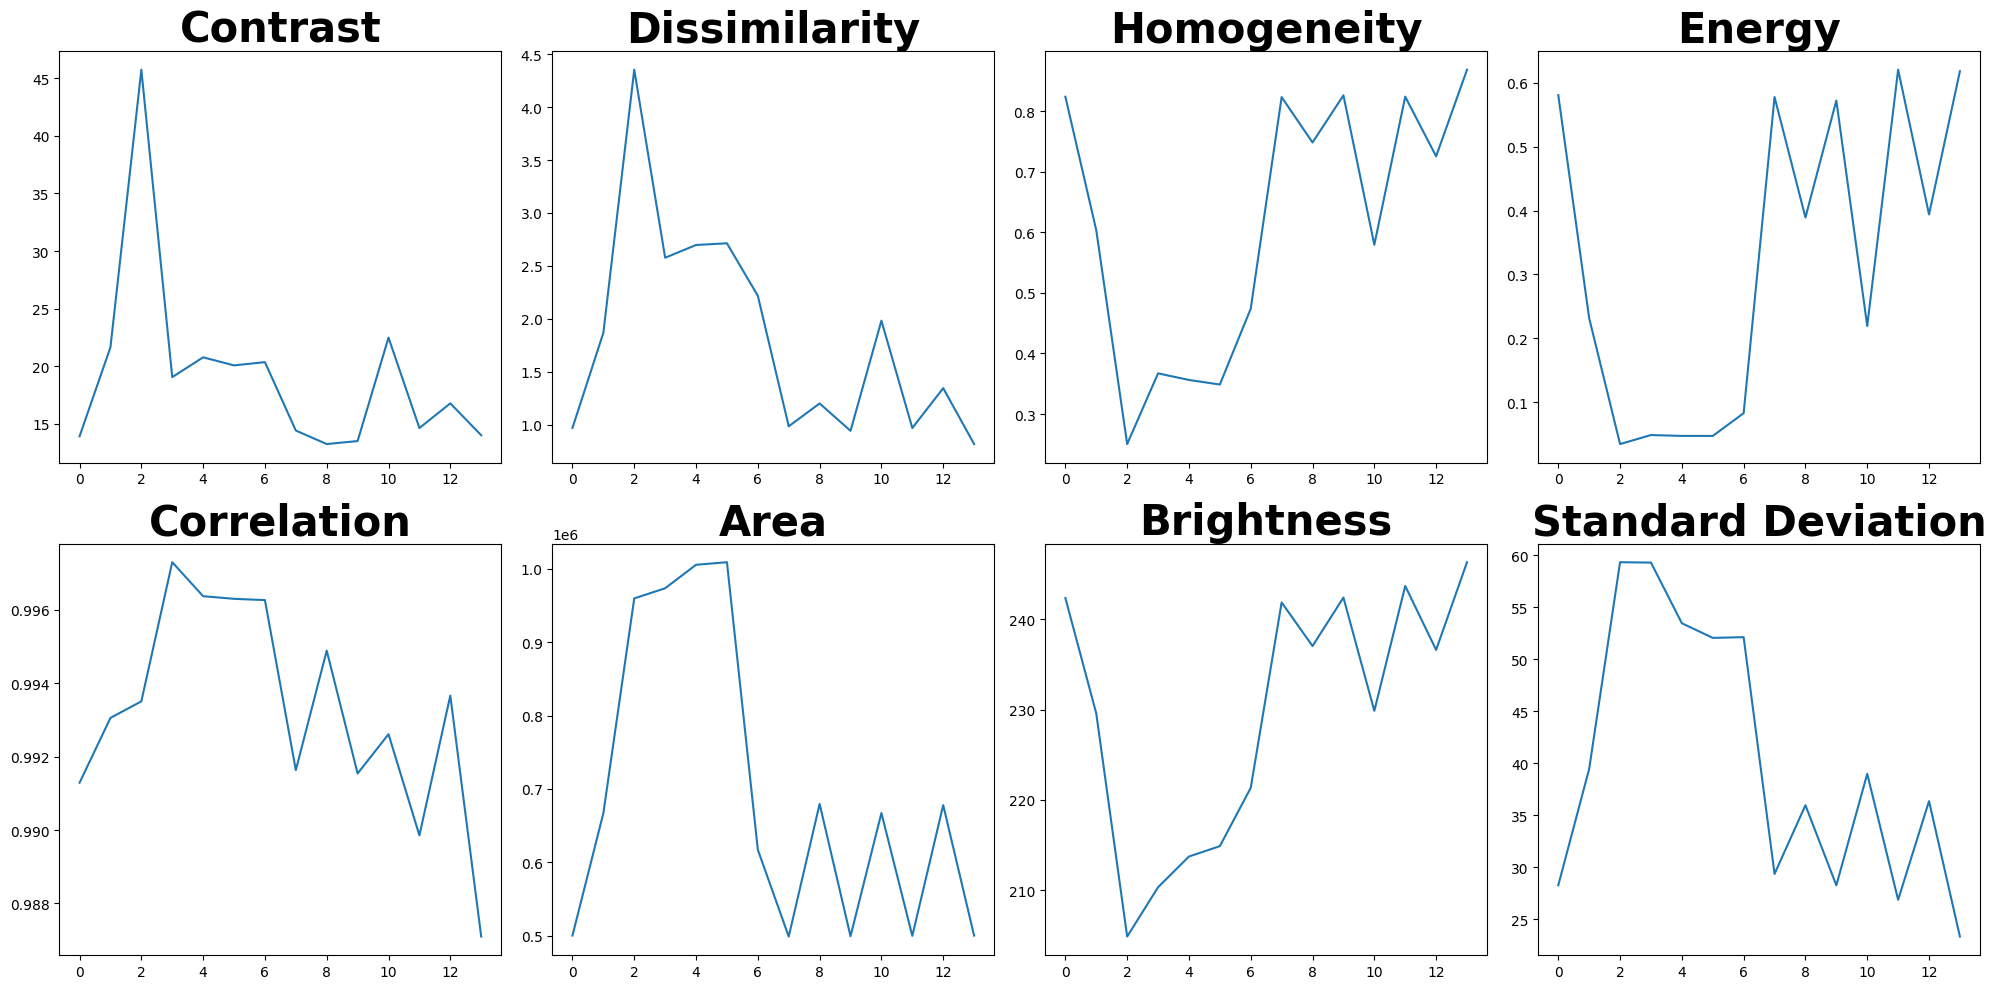
\includegraphics[width=\textwidth]{Figures/EDA_Charts/11/da.png}
        \caption*{Data Analysis}
    \end{minipage}
    \caption{Sipa 11 Analysis}
    \label{fig:Sipa 11 Analysis}
\end{figure}


\newpage


\section{Analysis Global Tesseract}

\subsection{First Run}

The first run performs Optical Character Recognition (OCR) on all of the images using the pytesseract library, a Python interface for the Tesseract OCR engine.

\begin{figure}[ht]
    \centering
    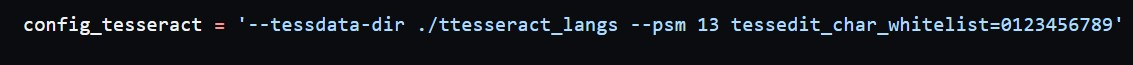
\includegraphics[width=0.9\textwidth]{Figures/firstrun/tesseract_config.jpg}
    \caption[PyTesseract Config Settings]{PyTesseract Config Settings}
    \label{fig:PyTesseract Config Settings}
\end{figure}


Firstly the libraries are imported for the analysis: numpy, pandas, and cv2 (OpenCV).

OCR is performed on the images using the configuration specified in Fig 3.11 above. Several variations of this configuration were tested and settings of PSM 6 and 7 were found to provide the good results, however 13 appears to provide the best results overall.

These results will be discussed in the Results chapter.

\newpage

\section{Analysis Tesseract Seperate Folders}


\subsection{Sipa 2}

\begin{figure}[ht]
    \centering
    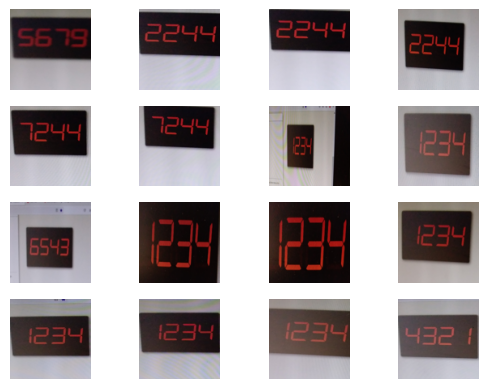
\includegraphics[width=0.9\textwidth]{Figures/EDA_Charts/2/montage.png}
    \caption[Sipa 2 Montage]{Sipa 2 Montage}
    \label{fig:Sipa 2 Montage}
\end{figure}


The Red Mask function operates on an input image to isolate and return only the red pixels in that image.

The input image should be a numpy ndarray representing the original image in BGR format. To process this, the function first converts the image into the HSV (Hue, Saturation, Value) colour space using OpenCV's cvtColor function.

Because the hue component of red colour in HSV space spans both ends of the hue spectrum, two ranges are defined to capture the entire red hue — the lower range (0-10) and the higher range (170-180). These ranges are combined with saturation and value thresholds to define what is considered a red pixel in the image.

The function then creates two binary masks for these ranges, using OpenCV's inRange function, which applies these boundaries on the HSV image. The resulting masks have pixel values of 255 where the original image pixels are within the specified red range, and 0 otherwise.

These two masks are added together to form a comprehensive mask of red pixels. The function then applies this mask onto a copy of the original image, setting all the pixels where the mask equals 0 to also be 0 in the output image. This leaves only the red pixels visible in the output image. Hence, the function returns an image emphasizing the red components of the original input.

\section{CRNN Training Databases}


\newpage

\begin{lstlisting}[language=Python, caption=Python example]
    def hello_world():
    print("Hello, world!")
\end{lstlisting}


the above code is a python code snippet.